\documentclass[11pt,psfig]{article}
\usepackage{epsfig}
\usepackage{times}
\usepackage{amssymb}
\usepackage{float}

\newcount\refno\refno=1
\def\ref{\the\refno \global\advance\refno by 1}
\def\ux{\underline{x}}
\def\uw{\underline{w}}
\def\bw{\underline{w}}
\def\ut{\underline{\theta}}
\def\umu{\underline{\mu}} 
\def\bmu{\underline{\mu}} 
\def\be{p_e^*}
\newcount\eqnumber\eqnumber=1
\def\eq{\the \eqnumber \global\advance\eqnumber by 1}
\def\eqs{\eq}
\def\eqn{\eqno(\eq)}

 \pagestyle{empty}
\def\baselinestretch{1.1}
\topmargin1in \headsep0.3in
\topmargin0in \oddsidemargin0in \textwidth6.5in \textheight8.5in
\begin{document}
\setlength{\parskip}{1.2ex plus0.3ex minus 0.3ex}


\thispagestyle{empty} \pagestyle{myheadings} \markright{G}



\title{CS 266 Homework 3}
\author{Zachary DeStefano, PhD Student, 15247592}
\date{Due Date: April 24}

\maketitle

\vfill\eject

\section*{Problem 3.11}

For this problem, it could end up not being monotone because of a concave vertex in the polygon that would cause there to be more than two intersection points in a given direction. We will thus go through each of the concave vertices and determine which directions that the polygon is not monotone in given that vertex. This will give us an interval of angles. Once we get the union of the intervals, we will see if that covers $[0,\pi]$ and if not, then the polygon is monotone for some direction. \\
\\
Here is the algorithm:\\
1. Initialize R to be empty. \\
2. For each vertex that is concave:\\
- Call the line segments through them $l$ and $l'$ \\
- Draw the lines perpendicular to $l$ and $l'$ and call them $L$ and $L'$\\
- Find the angles of $L$ and $L'$ with the x-axis and call them $\theta$ and $\theta'$. \\
- Find the min and max of $\theta$ and $\theta'$ and call them $\theta_1$ and $\theta_2$. \\
- Add $[\theta_1,\theta_2]$ to R.\\
3. Take the union of all the intervals in R. \\
4. If $[0,\pi] \subseteq R$, then the polygon is not monotone. \\
Otherwise it is monotone. 

\begin{figure}[H]
\centering
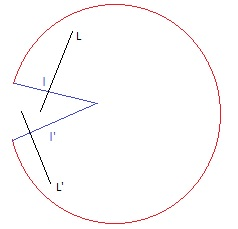
\includegraphics[height=3in]{monotone_diagram.jpg}
\caption{The non monotone directions with a concavity}
\end{figure}

Running time:\\
For each vertex, we do a constant number of operations. \\
Thus we have a total running time of $O(n)$

\newpage

\section*{Problem 3.14}

Given a simple polygon P with n vertices and a point p inside it, show
how to compute the region inside P that is visible from p.\\
\\
In the following figure, the visible region is the triangles with an X inside them. \\
\begin{figure}[H]
\centering
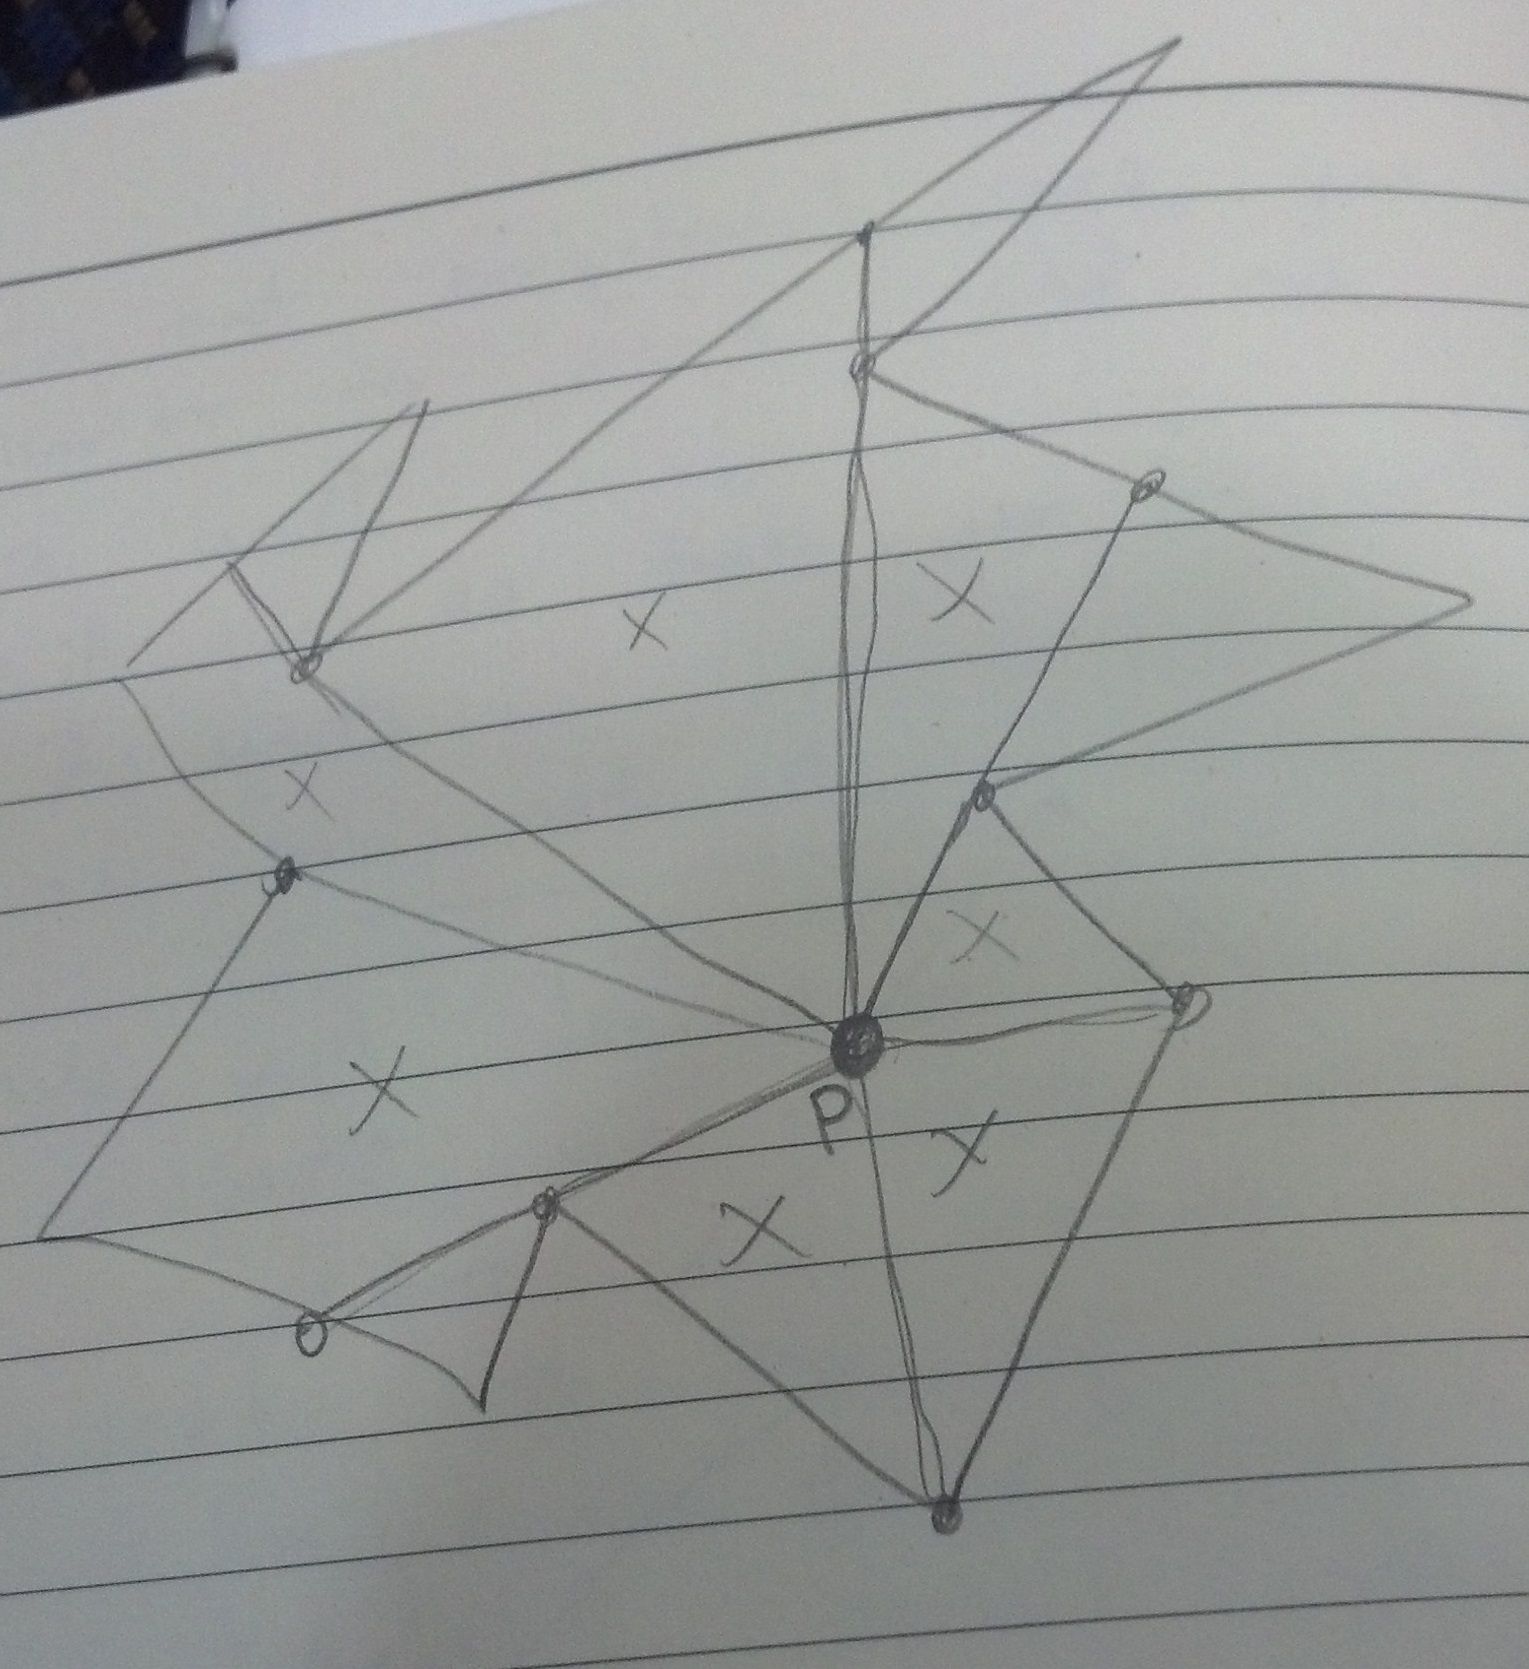
\includegraphics[height=4in]{visible_regions.jpg}
\caption{Parts of polygon visible from point p}
\end{figure}

The following procedure will be used:\\
For each vertex v with unobstructed view of p:\\
- Construct line segment from p, then passing through v, and ending at the next line segment in that direction. \\
- All the triangles that have just been constructed that are around p are the visible region. 

\newpage

\section*{Problem 15.2}

Algorithm VISIBILITYGRAPH calls algorithm VISIBLEVERTICES with
each obstacle vertex. VISIBLEVERTICES sorts all vertices around its
input point. This means that n cyclic sortings are done, one around each
obstacle vertex. In this chapter we simply did every sort in O(nlogn)
time, leading to O($n^2$ logn)time for all sortings. Show that this can be
improved to O($n^2$) time using dualization (see Chapter 8). Does this
improve the running time of VISIBILITYGRAPH?\\
\\
Idea:\\
Take the vertices and dualize them. \\
Construct the arrangement of the resulting lines. \\
Something in the arrangment tells you about how to construct the visibility graph

\newpage

\section*{Problem 15.4}

What is the maximal number of shortest paths connecting two fixed
points among a set of n triangles in the plane?\\
\\
The visibility graph will have $V = (3n+2)$.\\
For each vertex $v$ we have $|v| \leq 3n + 2$ for the number of vertices it is connected to. \\
The max number of paths is the max number of sequences of such vertices. \\
We need to start with $s$ and end with $t$ but the vertices in the middle do not matter. \\
We end up with $(3n)!$ paths possible. 


\end{document}








